\section{Reducing the Chains-Division Problem to the Assignment Problem}
In this section, we will show how we can reduce the problem of finding the optimal partition of the nodes of a labeled tree $T$ given their equivalence classes into $p$ chains to the Minimum Weight Perfect Bipartite Matching problem (see \cref{def:mwpbm}). We define \equivsetmath as the set of equivalence classes of the nodes of $T$, and $t$ as the number of nodes of the tree. This reduction will allow us to solve the problem in polynomial time, as shown in the previous chapter.

Then, we will show how to optimize the reduction by introducing some constraints that will allow us to reduce the number of edges in the bipartite graph, and we will also show how to move from the Minimum Weight Perfect Bipartite Matching problem to the more studied Maximum Weight Perfect Bipartite Matching problem without losing generality.

\subsection{\textsc{CHAINS-DIVISION} problem definition}
It is essential to begin by defining the problem we aim to solve.

\begin{definition}[\textsc{CHAINS-DIVISION} problem] \label{def:problem_def}
    Given a labeled tree $T$, the equivalence classes \equivsetmath, the stable order of the nodes in $T$ according to the upward path $\pi$ as defined in \cref{def:upward_path_sort}, and an integer parameter $p \in [2, t]$, find the optimal partition of the nodes of $T$ into $p$ chains such that the run-length encoding of each chain is minimized.
\end{definition}

Let's give a formal definition of run-length encoding.
\begin{definition}[Run length encoding]
    Given a sequence $S = \{s_1, s_2, \dots, s_n\}$, the run length encoding of $S$ is the sequence $R = \{r_1, r_2, \dots, r_m\}$ where $r_i$ is the number of times the element $s_i$ is repeated in $S$.
\end{definition}

It allows us to represent the sequence $S$ in a more compact way. \alessio{Metti un esempio, del RLE, magari anche del CDP.}

So, we aim to divide the nodes of the tree into $p$ chains such that the run-length encoding of the chains is minimized, meaning we want to reduce the number of distinct equivalence classes in each chain. Follows the definition of a chain.

\begin{definition}[Chains] \label{def:chains}
    Given a tree $T$, a chain $C$ is a sequence of nodes $C = \{c_1, c_2, \dots, c_m\}$ such that $C\subseteq V$. Additionally, each node of $T$ belongs to exactly one chain, and the nodes in the chain are ordered according to the upward path $\pi$ (as defined in \cref{def:upward_path_sort}) of each node $c_i$.
\end{definition}
\alessio{È abbastanza questa definizione? Se ho un albero con una radice A e due figli B e C, seguendo questa definizione, \{B, C\} è una catena, ma non sono comparabili e non possono generalmente. Penso che serva aggiungere che $c_i$ è genitore (o antenato) di $c_{i+1}$} 
\davide{effettivamente due nodi fratelli non sono comparabili ma da definizione di XBWT lo diventano in quanto l’algoritmo ordina in maniera stabile i nodi quindi rispettando l'ordinamento dei figli di un nodo (il figlio più piccolo nell'ordinamento è quello tutto a sx). Devo specificare meglio che la strategia di ordinamento utilizzata è quella specifica ottenuta con il pathSort così ogni incongruenza dovrebbe risolversi.. Corretto?}
\alessio{Ok, metterei una nota sotto la definizione specificando questa cosa allora. ``Note that, following the XBWT definition, two sibling nodes...''}

\subsection{Reduction idea}
The intuition behind the reduction is the following: given a tree $T$ and the number of chains $p$, we can construct a bipartite graph $G = (V, E)$ in which a perfect matching (\cref{def:matching}) always exists\draft{\sout{and, a}. In turn, a} perfect matching with minimum weight allows us to retrieve the optimal partition of the nodes of $T$ into $p$ chains such that the run-length encoding of each chain is minimized.

In the following sections we will show how to construct the bipartite graph $G$ and proof that $G$ constructed as defined in \cref{def:bip_construction} always allows to find a perfect matching and the weight of the matching is the minimum run length encoding of the optimal partition of the nodes of $T$ into $p$ chains.

\alessio{Introduci il bipartite graph con troppa cattiveria :). Prima abbiamo parlato di alberi, adesso subito di grafi bipartiti. La soluzione con grafo bipartito è quella che hai voluto seguire tu, quindi dovresti introdurla più come una scelta implementativa, che come un dato di fatto. In breve, dovresti dimostrare qua che Chains-Div. si riduce al MWBGP, quindi sarebbe da girare un attimo l'ordine: Se abbiamo un grafo con un perfect matching allora possiamo ridurre il problema -> creiamo un grafo in questo modo -> contiene un perfect matching -> possiamo sempre fare la riduzione.} \davide{Ho aggiunto un paragrafo introduttivo.. può andare o intendevi proprio girare tutta la dimostrazione?}
\alessio{Se l'esistenza perfect matching è sufficiente a fare la riduzione, secondo me è meglio girare l'ordine delle dimostrazioni. Altrimenti, se per la riduzione ti servono le proprietà specifiche del grafo che hai creato allora va bene questo ordine. Pensandoci, puoi riportare questa discussione nell'intrduzione della sezione 6.2, mettendo qualcosa tipo ``In particular we show that, given a tree $T$ and the number of chains $p$, we can construct a bipartite ...'' tra i due paragrafi che ci sono già. (occhio alle frasi troppo lunghe).}

\subsection{Bipartite graph construction}
Now, we will show how to construct a bipartite graph that allows us to solve the \textsc{CHAINS-DIVISION} problem.

\begin{definition}[Bipartite graph construction] \label{def:bip_construction}
    Let $T$ be a tree with $t$ nodes, and $p$ the number of chains we want to partition the nodes into. Let \equivsetmath be the set of equivalence classes of the nodes of $T$. We can construct a bipartite graph $G = (V, E)$ such that vertices are divided in two disjoint sets $V = V_1 \cup V_2$ in the following way:
    \begin{itemize}
        \item $V_1$ contains $t + p$ nodes composed by $p$ source nodes $s_1, s_2, \dots, s_p$ (referred to collectively as \sourceset) followed by the $t$ elements (referred to collectively as \treeset{V_1}) of \equivsetmath. The nodes in $V_1$ follow a strict ordering $s_1 \prec s_2 \prec \dots \prec s_p \prec u_1 \prec u_2 \prec \dots \prec u_t$, where $u_i$ are the tree nodes ordered according to the upward path $\pi$ as defined in \cref{def:upward_path_sort}. 
        \item $V_2$ contains $t + p$ nodes composed by the $t$ elements (referred to collectively as \treeset{V_2}) of \equivsetmath followed by $p$ destination nodes $d_1, d_2, \dots, d_p$ (referred to collectively as \destset). The nodes in $V_2$ follow a strict ordering $v_1 \prec v_2 \prec \dots \prec v_t \prec d_1 \prec d_2 \prec \dots \prec d_p$, where $v_i$ are the tree nodes ordered according to the upward path $\pi$ as defined in \cref{def:upward_path_sort}.
    \end{itemize}

    Then the edges of the graph $G$ are constructed in the following way:
    \begin{enumerate}
        \item The \sourceset nodes are connected to the first $p$ nodes with distinct equivalence class in $V_2$, with weight $1$.
        \item Let $u_i \in$ \treeset{V_1}. We define \equivsetfunc{u_i} as the equivalence class of node $u_i$. For each node $u_i$, we construct the following edges:
        
        - For the first $p$ nodes $v_j \in$ \treeset{V_2} such that $j > i$ and \equivsetfunc{v_j} $\neq$ \equivsetfunc{u_i}, we add an edge $(u_i, v_j)$ with weight $1$. If there are fewer than $p$ nodes in $V_2$ with distinct equivalence classes, we stop earlier.

        - Let $v_k \in$ \treeset{V_2} be the first node in the ordering such that $k > i$ and \equivsetfunc{v_k} $=$ \equivsetfunc{u_i}, we add an edge $(u_i, v_k)$ with weight $0$. If such a node does not exist, we add $p$ edges $(u_i, d_j)$ with weight $0$ for each $j = 1, 2, \ldots, p$, where $d_j \in$ \destset.
    \end{enumerate}
    \alessio{Bella!}
\end{definition}

Notice that it is important to consider the order of the nodes of the two sets $V_1$ and $V_2$ as stated in the definition, because we will need to connect the source nodes to the destination nodes in a way that will allow us to find the optimal partition of the nodes of the tree. An example of the node structure is shown in \cref{fig:reduction_example_parts}.

Notice also that when we talk about the same \treeset{V_1} node placed in \treeset{V_2}, we are referring to the corresponding node in \treeset{V_2} that derives from the same node in the original tree $T$ since the nodes of the tree are ordered in both sets \treeset{V_1} and \treeset{V_2}. In  \cref{fig:reduction_example_parts,fig:reduction_small_examples,fig:reduction_example}, the node's correspondence is achieved by putting the two nodes at the same level.

\begin{figure}[H]
    \centering
    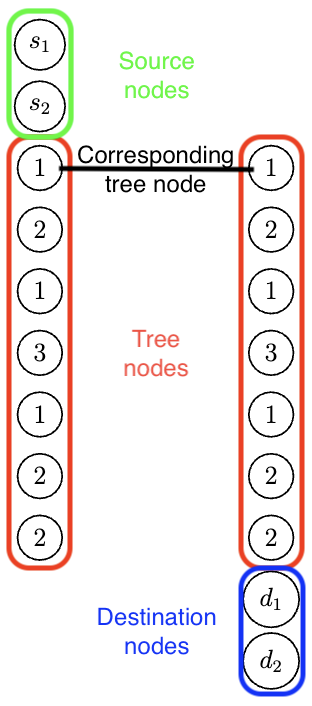
\includegraphics[width=0.3\textwidth]{Immagini/bipartite_keys_part.png}
    \caption[Bipartite nodes structure]{Example of a bipartite graph nodes constructed from a tree with the following equivalence classes $E = \{1,2,1,3,1,2,2\}$. The nodes are ordered from top to bottom. \alessio{Che ne pensi di mettere l'albero di partenza nell'immagine? (usando le Eq. class, non i valori originali)}}
    \alessio{Altra cosa, nel capitolo 4 le classi di equivalenza sono nominate con lettere maiuscole. Penso che sarebbe meglio usare la stessa notazione, così non ci si confonde sul fatto che i numeri non sono quantità.}
    \label{fig:reduction_example_parts}
\end{figure}

Let's see a small example for each case, consider $p=2$. In \cref{fig:reduction_small_examples}-(a), there is an example for the sources' edges. As stated before, for each source, $p$ edges with weight $1$ are created and connected to the first $p$ nodes with distinct equivalence class in \treeset{V_2}.

In \cref{fig:reduction_small_examples}-(b), there is an example for the tree nodes' edges. For each node in \treeset{V_1}, edges with weight $1$ are created and connected to the first $p$ nodes with distinct equivalence class in \treeset{V_2}, after the corresponding node in \treeset{V_2} (coming after the node itself in the ordering), and edges with weight $0$ are created and connected to the first node with the same class in \treeset{V_2} after the corresponding node in \treeset{V_2}. As we can see from the image, we consider the first node in \treeset{V_1} labelled $1$ that is connected to the node $2$ with weight $1$, and to the node $3$ with weight $1$, and to the second node labelled $1$ in $V_2$ with weight $0$.

Lastly, in \cref{fig:reduction_small_examples}-(c) there is an example for the destination nodes' edges. We start by considering the node in \treeset{V_1} that is labelled $1$, which is connected to node $2$ with weight $1$. Then, since there is no node with the same class in \treeset{V_2}, we connect it to the destination nodes $d_1$ and $d_2$ with weight $0$. The same is done for the second node in $V_1$ that is labelled $2$ since no nodes are coming after it in the order; it is connected to the destination nodes $d_1$ and $d_2$ with weight $0$.

\begin{figure}[H]
    \centering
    \tikzset{main/.style = {draw, circle, thick, minimum size=8mm, inner sep=0pt}}

    \begin{subfigure}[b]{0.3\textwidth}
        \centering
        \begin{tikzpicture}[node distance=10mm, auto=center]
            % Left column (sources)
            \node[main] (1s) {$s_1$};
            \node[main] (2s) [below of=1s] {$s_2$};
            \node[main] (3s) [below of=2s] {$1$};
            \node[main] (4s) [below of=3s] {$1$};
            \node[main] (5s) [below of=4s] {$2$};
            \node (dots_s) [below of=5s] {\vdots}; % Vertical dots

            % Right column (destinations)
            \node[main] (1d) [right=2.5cm of 3s] {$1$};
            \node[main] (2d) [below of=1d] {$1$};
            \node[main] (3d) [below of=2d] {$2$};
            \node (dots_d) [below of=3d] {\vdots}; % Vertical dots

            % Arrows
            \draw[red, ->] (1s) -- (1d);
            \draw[red, ->] (1s) -- (3d);
            \draw[red, ->] (2s) -- (1d);
            \draw[red, ->] (2s) -- (3d);
        \end{tikzpicture}
        \caption{}
        \label{fig:sub1}
    \end{subfigure}
    \hfill % Space between subfigures
    \begin{subfigure}[b]{0.3\textwidth}
        \centering
        \begin{tikzpicture}[node distance=10mm, auto=center]
            % Left column (tree nodes)
            \node (dots_s_top) {\vdots};
            \node[main] (3s) [below of=dots_s_top] {$1$};
            \node[main] (4s) [below of=3s] {$2$};
            \node[main] (5s) [below of=4s] {$1$};
            \node[main] (6s) [below of=5s] {$3$};
            \node (dots_s_bottom) [below of=6s] {\vdots};

            % Right column (destinations)
            \node (dots_d_top) [right=2.5cm of dots_s_top] {\vdots};
            \node[main] (1d) [below of=dots_d_top] {$1$};
            \node[main] (2d) [below of=1d] {$2$};
            \node[main] (3d) [below of=2d] {$1$};
            \node[main] (4d) [below of=3d] {$3$};
            \node (dots_d_bottom) [below of=4d] {\vdots};

            % Arrows
            \draw[red, ->] (3s) -- (2d);
            \draw[red, ->] (3s) -- (4d);
            \draw[green, ->] (3s) -- (3d);
        \end{tikzpicture}
        \caption{}
        \label{fig:sub2}
    \end{subfigure}
    \hfill % Space between subfigures
    \begin{subfigure}[b]{0.3\textwidth}
        \centering
        \begin{tikzpicture}[node distance=10mm, auto=center]
            % Left column (original destinations)
            \node (dots_s_top) {\vdots};
            \node[main] (7s) [below of=dots_s_top] {$1$};
            \node[main] (9s) [below of=7s] {$2$};

            % Right column (bipartite graph destinations)
            \node (dots_d_top) [right=2.5cm of dots_s_top] {\vdots};
            \node[main] (5d) [below of=dots_d_top] {$1$};
            \node[main] (6d) [below of=5d] {$2$};
            \node[main] (8d) [below of=6d] {$d_1$};
            \node[main] (9d) [below of=8d] {$d_2$};

            % Arrows
            \draw[red, ->] (7s) -- (6d);
            \draw[green, ->] (7s) -- (8d);
            \draw[green, ->] (7s) -- (9d);
            \draw[green, ->] (9s) -- (8d);
            \draw[green, ->] (9s) -- (9d);
        \end{tikzpicture}
        \caption{}
        \label{fig:sub3}
    \end{subfigure}

    \caption[Examples of reduction to a bipartite graph]{Examples of the connection construction in the bipartite graph for $p=2$, showing the cases for source nodes \sourceset (a), internal tree nodes \treeset{V_1} and \treeset{V_2} (b), and destination nodes \destset (c). Red arrows indicate edges with weight 1, while green arrows indicate edges with weight 0.}
    \label{fig:reduction_small_examples}
\end{figure}

Before we present the proof of the correctness of the reduction, let us state the following theorem regarding the number of edges in the bipartite graph resulting from \cref{def:bip_construction}. This theorem is essential for understanding the complexity of the final algorithm employed to solve the \textsc{MWPBM} problem and so, the \textsc{CHAIN-DIVISION} problem.

\begin{theorem}[Bipartite graph properties]
    The bipartite graph $G$ constructed as stated in \cref{def:bip_construction} has $2t + 2p$ nodes and $O(t (p + 1) + p^2 + tp)$ edges.
\end{theorem}

\begin{proof}
    The $O(t (p + 1))$ edges come from the tree nodes, the $O(p^2)$ edges come from the sources since each source node is connected to $p$ nodes, and the $O(tp)$ edges come from the destination nodes since in the worst case we have $t$ distinct equivalence class and so all the nodes are connected to the destination nodes. 
\end{proof}

\subsection{Proof of correctness}
In this section, we present the proof of the correctness of the reduction introduced in the previous sections. Let's start by stating the following lemmas.

\begin{lemma} \label{lemma:all_destinations}
    Exactly $|\equivset|$ nodes of the set \treeset{V_1} are connected to all the destination nodes $d_i \in$ \destset with weight $0$.
\end{lemma}

\begin{proof}
    As outlined in \cref{def:bip_construction}, the destination nodes $d_i \in V_2$ are connected to nodes $u_i \in$ \treeset{V_1} with weight $0$ iff \draft{\sout{there is no other node} for all} $v_j \in$ \treeset{V_2} such that $j \draft{>} i$ \alessio{È giusto o dovrebbe essere $<$?} \draft{\sout{and},} \equivsetfunc{v_j} $\neq$ \equivsetfunc{u_i}, \draft{\sout{meaning that they are} i.e. $u_i$ is the} last of \draft{\sout{their} its} class in the ordering. Consequently, there are exactly $|\equivset|$ nodes in \treeset{V_1} that are last representatives of their class in the ordering.
    \alessio{``no other'' e ``$\neq$'' creano una doppia negazione, quindi si traduce in "se ci sono altri nodi che hanno una classe di equivalenza uguale." Quello che vuoi dire qua è che, dato un nodo $u$, questo si connette alle destinazioni sse tutti gli altri nodi hanno una classe di equivalenza diversa da $u$ (o posta al contrario, se nessun nodo dopo ha classe equivalenza uguale). Le negazioni in italiano sono un casino...}
\end{proof}

\begin{lemma} \label{lemma:optimal_cost}
    The optimal solution of an instance $\mathcal{I}$ of the \textit{CHAINS-DIVISION} problem for a tree $T$ is always greater than or equal to $|\equivset|$.
\end{lemma}

\begin{proof}
    To minimize the run-length encoding of the chains, we note that the minimum cost of a chain is $1$. Consequently, the optimal cost of the \textit{CHAINS-DIVISION} problem for the tree $T$ is always greater than or equal to the cardinality of the set of equivalence classes \equivsetmath. This is because if we partition them into $p = |\equivset|$ chains, the cost will be equal to $|\equivset|$, since each chain contains only nodes belonging to the same class. Conversely, if we partition them into $p < |\equivset|$ chains, the cost will be greater than or equal to $|\equivset|$, since we will need to include at least two nodes from different classes within a single chain \draft{\sout{or more}}.
\end{proof}

\begin{claim} \label{claim:p_less_than_E}
    The solutions for the \textit{CHAINS-DIVISION} problem for the instances where the number $p$ of chains is greater than $|\equivset|$ are not better than the solutions for the instances where $p \leq |\equivset|$.
\end{claim}

\begin{proof}
    The proof comes directly from \cref{lemma:optimal_cost}. \alessio{Magari spiega che appunto avresti chain vuote quindi la soluzione è cmq $|\equivset|$}
\end{proof}

Therefore, for the proof of the reduction, we will only consider instances of the problem where $p < |\equivset|$, as they do not present a trivial solution.

\begin{lemma} \label{lemma:greater_nodes}
    Given a bipartite graph $G$ constructed as stated in \cref{def:bip_construction}, for each node $u_i \in$ \treeset{V_1} it is impossible for $u_i$ to be connected to a node $v_j \in$ \treeset{V_2}, such that $j < i$ in the order of the nodes.
    \alessio{Anche per $\leq$ dovrebbe andare bene, che è anche più stringente.}
\end{lemma}

\begin{proof}
    The proof comes from the construction of $G$ (\cref{def:bip_construction}) where the nodes of \treeset{V_1} are always connected to the nodes of \treeset{V_2} coming after them \draft{\sout{in the ordering of the nodes of the tree $T$}}.
\end{proof}

\alessio{Lo metterei come Lemma questo piuttosto che come claim. Come per il Claim 1, dovrebbero derivare direttamente da un altro lemma.}
\begin{claim} \label{claim:node_connectivity}
    In the bipartite graph $G$ constructed as per \cref{def:bip_construction}, for every node $u \in \treesetbase{V_1}$ \rem{has a non-empty neighborhood, i.e.} $|N(\{u\})| \geq 1$.
\end{claim}
\draft{In other words, every node in $V_1$ is connected to at least another node in $V_2$.}
\begin{proof}
    Let $u_i \in \treesetbase{V_1}$ be an arbitrary node. We analyze the construction of its outgoing edges based on \cref{def:bip_construction}. There are two mutually exclusive cases for $u_i$:
    \begin{enumerate}
        \item There exists at least one node $v_k \in \treesetbase{V_2}$ with $k > i$ that has the same equivalence class as $u_i$, i.e., \equivsetfunc{v_k} $=$ \equivsetfunc{u_i}. In this case, the construction specifies that an edge is added between $u_i$ and the first such node $v_k$. This guarantees $u_i$ has at least one neighbor.
        \item There are no nodes $v_k \in \treesetbase{V_2}$ with $k > i$ that share the same equivalence class as $u_i$. This occurs when $u_i$ is the last node of its equivalence class in the specified ordering. In this scenario, the construction adds $p$ edges from $u_i$ to each of the destination nodes $d_j \in \destsetbase$. Since $p \geq 2$, $u_i$ is connected to at least two nodes.
    \end{enumerate}
    In either case, any node $u_i \in \treesetbase{V_1}$ is guaranteed to have at least one outgoing edge. Therefore, its neighborhood is non-empty.
\end{proof}

\begin{lemma} \label{lemma:distinct_neighborhoods}
    For any pair of distinct nodes $u_i, u_j \in \treesetbase{V_1}$\rem{, their sets of neighbors are distinct, i.e.}, $N(\{u_i\}) \neq N(\{u_j\})$.
\end{lemma}
\begin{proof}
    Let $u_i, u_j \in \treesetbase{V_1}$ be two distinct nodes. Without loss of generality, assume $i < j$. \alessio{Dato che i nodi hanno un ordinamento, potresti lavorare direttamente su quelli, dicendo $u_i \prec u_j$, che implica anche l'ordinamento dei nodi dell'albero e non serve riscriverlo (vedi prima).}

    \draft{\sout{By Lemma 3, any neighbor of $u_j$ belonging to \treeset{V_2} must be a node $v_k$ with index $k > j$.}} \alessio{Questo lo ripeti sotto}

    Now consider node $u_i$. By \cref{claim:node_connectivity}, its set of neighbors $N(\{u_i\})$ is non-empty. Let $y$ be a neighbor of $u_i$. If $y$ is a node $v_k \in \treesetbase{V_2}$, then\draft{, by \cref{lemma:greater_nodes},} its index $k$ must be greater than $i$.

    If we can find a neighbor $v_k \in N(\{u_i\})$ with $k \leq j$, then the proof is complete, since\draft{, following \cref{lemma:greater_nodes},} $v_k$ cannot be a neighbor of $u_j$. Let's assume by contradiction that every neighbor $v_k \in N(\{u_i\})$ has an index $k > j$. This would imply that $u_i$ is not connected to any node $v_k$ with $i < k \leq j$.

    However, consider node $v_{i+1}$. Since $i < t$ (otherwise $j$ would not exist), this node exists. Given that $i < i+1 \leq j$ (since $j$ is an integer and $j>i$), our hypothesis implies that $v_{i+1}$ cannot be a neighbor of $u_i$. Let's analyze why this would be impossible:
    \begin{itemize}
        \item If \equivsetfunc{v_{i+1}} $=$ \equivsetfunc{u_i}, then by construction $u_i$ must be connected to $v_{i+1}$ (the first subsequent node with the same class). This contradicts our hypothesis.
        \item If \equivsetfunc{v_{i+1}} $\neq$ \equivsetfunc{u_i}, then $v_{i+1}$ is the first candidate to be a neighbor with a different class. By construction, $u_i$ is connected to the first $p$ nodes with different classes, so $v_{i+1}$ must be in $N(\{u_i\})$ (since $p \geq 1$). This also contradicts our hypothesis.
    \end{itemize}
    In both cases, we arrive at a contradiction. Therefore, the initial hypothesis must be false. There must exist at least one neighbor $v_k$ of $u_i$ with $i < k \leq j$. Since $k \leq j$, $v_k$ cannot be a neighbor of $u_j$. Consequently, $N(\{u_i\}) \neq N(\{u_j\})$.
\end{proof}

\begin{claim} \label{claim:prev_not_subset}
    For any pair of distinct nodes $u_i, u_j \in \treesetbase{V_1}$ with $i < j$, then we have that $N(\{u_i\}) \not\subseteq N(\{u_j\})$.
\end{claim}
\begin{proof}
    This is a direct consequence of the proof of \cref{lemma:distinct_neighborhoods}. In that proof, we showed that for any pair of nodes $u_i, u_j$ with $i < j$, there exists a neighbor $v_k \in N(\{u_i\})$ such that $k \leq j$. By \cref{lemma:greater_nodes}, any neighbor of $u_j$ must have an index greater than $j$. Therefore, $v_k$ cannot be a neighbor of $u_j$, which implies that $N(\{u_i\})$ cannot be a subset of $N(\{u_j\})$.
\end{proof}

\begin{lemma} \label{lemma:matching_existence}
    For every possible instance of the \textit{CHAINS-DIVISION} problem, a perfect matching exists in the bipartite graph G constructed as specified in \cref{def:bip_construction}.
\end{lemma}

\begin{proof}
    The proof comes from the construction of the bipartite graph $G$ and from \cref{thm:halls_marriage_theorem}. We are going to prove that $G$ satisfies Hall's condition (see \cref{thm:halls_marriage_theorem}) and so, since by construction $|V_1| = |V_2|$, a perfect matching for $G$ exists.

    To verify Hall's condition, we need to prove that for any subset $W \subseteq V_1$ we have that $|N(W)| \geq |W|$, where $N(W)$ is the neighborhood of $W$ (\cref{def:neighborhood}). We have the following cases:
    \begin{enumerate}
        \item $W \subseteq$ \sourceset: Let $W$ be a subset of $S$ of size $k$. By construction, every source node $s_i \in$ \sourceset is connected to the same set of $p$ nodes in $V_2$, which are the first $p$ nodes with distinct equivalence classes in the ordering. Therefore, for any non-empty $W \subseteq$ \sourceset, the neighborhood $N(W)$ consists of exactly these $p$ nodes, so $|N(W)| = p$. From \cref{lemma:optimal_cost} and \cref{claim:p_less_than_E}, we only consider instances where $p \leq |\equivset|$, ensuring that at least $p$ such nodes exist. Since $|\sourcesetbase|=p$, we have $|W| = k \leq p$. Thus, $|N(W)| \geq |W|$.
        
        \item $W \subseteq$ \treeset{V_1}: Let $W = \{u_{i_1}, \dots, u_{i_k}\} \subseteq \treesetbase{V_1}$ with $i_1 < i_2 < \dots < i_k$. We prove by induction on $k = |W|$ that $|N(W)| \geq |W|$.
        
        \textbf{Base case ($k=1$):} Let $W = \{u_{i_1}\}$. By \cref{claim:node_connectivity}, $N(W)$ is not empty, so $|N(W)| \geq 1 = |W|$.
        
        \textbf{Inductive step:} Assume the property holds for any subset of size $k-1$. Let $|W|=k$. Let $W' = W \setminus \{u_{i}\}$. By the inductive hypothesis, $|N(W')| \geq k-1$. By \cref{claim:prev_not_subset}, for any two nodes $u_a, u_b \in \treesetbase{V_1}$ with $a < b$, we have $N(\{u_a\}) \not\subseteq N(\{u_b\})$. Since $u_{i_k}$ is the node with the lower index in $W$, this property implies that $N(\{u_{i_k}\}) \neq N(W')$. This means there exists at least one node $y \in N(\{u_{i_k}\})$ such that $y \notin N(W')$. Therefore, $|N(W)| = |N(W') \cup N(\{u_{i_k}\})| \geq |N(W')| + 1 \geq (k-1) + 1 = k$.

        Thus, for any $W \subseteq \treesetbase{V_1}$, Hall's condition $|N(W)| \geq |W|$ is satisfied.
        
        \item $W=W_S \cup W_U$, where $W_S \subseteq \sourcesetbase, W_U \subseteq \treesetbase{V_1}$: We have $|N(W)| \geq |W|$ as a derivation from the previous cases and \cref{lemma:greater_nodes}.
    \end{enumerate}
\end{proof}

\alessio{Questa parte non mi convince ancora. Penso che se dimostrassi il lemma che ogni nodo in $U$ punta almeno ad un nodo diverso dagli altri, tutti questi punti non servono, ma non saprei ancora come dimostrarlo...} \davide{Ho seguito questa strada, fammi sapere se secondo te è corretto il lemma che ho aggiunto.}

\alessio{Un lemma è utile perché è un mini teorema che serve a dimostrare un teorema più grande. Se enunci dei lemmi prima di un teorema, dovresti usarli all'interno della sua dimostrazione.} \davide{Attualmente solo il lemma 1 non viene utilizzato. Lo tolgo?}

\begin{comment}
    \begin{proof}
        The proof comes from the construction of the bipartite graph $G$ and from theorem \cref{thm:perfect_matching_existence}. We are going to proof that the bipartite graph $G$ constructed as stated in \cref{def:bip_construction} has a Tutte matrix (\cref{def:tutte_matrix}) with determinant different from $0$ and so a perfect matching for $G$ exists.

        We know that a $n \times n$ matrix $M$ has $Det(M) \neq 0$ if and only if it has full rank ($rank(M) = n$), or equivalently if it has $n$ linearly independent rows or columns. We can see that the bipartite graph $G$ has $2t + 2p$ nodes and $O(t (p + 1) + p^2 + tp)$ edges, and so the Tutte matrix of $G$ will have $2t + 2p$ rows and $2t + 2p$ columns. The columns of $M$ are all independent since each node of $G$ in $V_1$ is connected only to nodes in $V_2$ that are greater than $u$ in the ordering. Also each node is connected to at least one node in $V_2$ and at most $p + 1$ distinct nodes with distinct class in $V_2$. Those conditions on the edges are sufficient to get a full rank matrix and so a perfect matching for $G$ exists.
    \end{proof}

    In \cref{fig:tutte_matrix_ex} the Tutte matrix for the bipartite graph in \cref{fig:reduction_example}-(a) is shown.

    \begin{figure}
        \centering
        \[
        \begin{array}{c|ccccccccc}
                & \text{1} & \text{2} & \text{1} & \text{3} & \text{1} & \text{2} & \text{2} & \text{$d_1$} & \text{$d_2$} \\
            \hline
            \text{$s_1$} & 1 & 1 & 0 & 0 & 0 & 0 & 0 & 0 & 0 \\
            \text{$s_2$} & 1 & 1 & 0 & 0 & 0 & 0 & 0 & 0 & 0 \\
            \text{1}     & 0 & 1 & 1 & 1 & 0 & 0 & 0 & 0 & 0 \\
            \text{2}     & 0 & 0 & 1 & 1 & 0 & 1 & 0 & 0 & 0 \\
            \text{1}     & 0 & 0 & 0 & 1 & 1 & 1 & 0 & 0 & 0 \\
            \text{3}     & 0 & 0 & 0 & 0 & 1 & 1 & 0 & 1 & 1 \\
            \text{1}     & 0 & 0 & 0 & 0 & 0 & 1 & 0 & 1 & 1 \\
            \text{2}     & 0 & 0 & 0 & 0 & 0 & 0 & 1 & 0 & 0 \\
            \text{2}     & 0 & 0 & 0 & 0 & 0 & 0 & 0 & 1 & 1 \\
        \end{array}
        \]
        \caption[Tutte matrix example]{Example of a Tutte matrix for a bipartite graph in \cref{fig:reduction_example}-(a). As we can see the matrix has full rank and so a perfect matching exists.}
        \label{fig:tutte_matrix_ex}
    \end{figure}
\end{comment}

We can now prove the correctness of the reduction. Consider a perfect matching $M$ in $G$. Therefore, $|V_1|=|V_2|$ and $M$ is perfect, every node in $V_1$ is matched to exactly one node in $V_2$, and vice versa. The matching $M$ consists of $t+p$ edges. Due to the construction of $G$ (\cref{def:bip_construction}) and \cref{lemma:greater_nodes} (a node $u_i \in \treesetbase{V_1}$ only connect to a node $v_j \in \treesetbase{V_2}$ with $i < j$ or to destination nodes \destset), the matching $M$ naturally decomposes into $p$ paths starting from the source nodes $s_1, \dots, s_p$ and ending at the destination nodes $d_1, \dots, d_p$. Each path traverses a sequence of nodes corresponding to the nodes of the original tree $T$.
Specifically, a path starting at $s_i$ will match it to a node $u_{a} \in \treesetbase{V_2}$. Then, the corresponding node of $u_{a} \in \treesetbase{V_1}$ can be matched to a node $u_{b} \in \treesetbase{V_2}$ (where $b > a$). This continues until a node $u_{x} \in \treesetbase{V_1}$ is matched to a destination node $d_k \in \destsetbase$. This forms a sequence $s_i \rightarrow u_{a} \rightarrow u_{b} \rightarrow \dots \rightarrow u_{x} \rightarrow d_k$. Following this technique, we will retrieve all the optimal chains from the solution of the \textsc{MWPBM} problem.

\alessio{Tutta questa parte qua la spiegherei prima, fuori da questa dimostrazione. È importante per definire bene il problema e in questo modo snellisci anche la proof.} \davide{l'ho spostata qui. TODO: aggiungere esempio grafico}

\begin{theorem}
    An optimal solution of an instance $\mathcal I$ with $p \leq |\equivset|$ of the \textsc{CHAINS-DIVISION} problem (\cref{def:problem_def}) is equivalent to an optimal solution of the \textsc{MWPBM} problem (\cref{def:mwpbm}) for the instance $r(\mathcal I)$ where $r: \mathcal{I}_{CHAINS-DIVISION} \rightarrow \mathcal{I}_{MWPBM}$ is the reduction function that maps an instance of the CHAINS-DIVISION problem to an instance of the MWPBM problem for a bipartite graph $G$ constructed as stated in \cref{def:bip_construction}.
\end{theorem}

\begin{proof}
    Let $\mathcal{I} = (T, \equivset, p)$ be an instance of the \textsc{CHAINS-DIVISION} problem, where $T$ is a tree with $t$ nodes, \equivsetmath is the set of equivalence classes, and $p$ is the target number of chains. We assume $p \leq |\equivset|$, per \cref{claim:p_less_than_E}. Let $G = r(\mathcal{I})$ be the bipartite graph constructed according to \cref{def:bip_construction}. We will demonstrate a bijection between the set of valid chain partitions of $T$ and the set of perfect matchings in $G$, such that the cost of a partition equals the weight of its corresponding matching.

    First, we establish the existence of a perfect matching. By construction, the graph $G$ is bipartite with partitions $V_1$ and $V_2$ such that $|V_1| = |V_2| = t+p$. \cref{lemma:matching_existence} ensures that a perfect matching exists in $G$.

    Let $\mathcal{P} = \{C_1, \dots, C_p\}$ be a valid partition of the nodes of $T$ into $p$ chains. We can construct a perfect matching $M_\mathcal{P}$ in $G$ as follows:  For each chain $C_k = [u_{1}, \dots, u_{m_k}]$, we construct a path in $G$: match $s_k$ to $u_{1} \in \treesetbase{V_2}$. Then match $u_{i} \in \treesetbase{V_1}$ to $u_{i+1} \in \treesetbase{V_2}$ for $i=1, \dots, m_k-1$. Finally, match $u_{m_k} \in \treesetbase{V_1}$ to one of the available destination nodes $d_j \in \destsetbase$. Since we have $p$ chains and $p$ source/destination nodes, and every tree node is in exactly one chain, this process uses all $t+p$ nodes in $V_1$ and $V_2$, forming a perfect matching. The weight of this matching is given by:
    \begin{align*}
        W(M_\mathcal{P}) &= \sum_{(u,v) \in M_\mathcal{P}} w(u,v) \\
        &= p + |\{ (u_i, u_j) \in M_\mathcal{P} \mid u_i \in \treesetbase{V_1}, u_j \in \treesetbase{V_2}, \equivset(u_i) \neq \equivset(u_j) \}|
    \end{align*}
    where $p$ represents the contribution from the source nodes $s_i$, as each source node must be connected with weight 1 to start a chain. A class change occurs exactly when a path in the matching uses a weight-1 edge between tree nodes.
    Therefore, $W(M)$ is exactly equal to the RLE cost of the partition defined by the matching $M_\mathcal{P}$.

    Conversely, let $M$ be a perfect matching in $G$. The structure of $G$ ensures that $M$ consists of $p$ disjoint paths starting from source nodes $\{s_1, \dots, s_p\}$ and ending at destination nodes $\{d_1, \dots, d_p\}$. Each path defines an ordered chain of nodes from $T$. By \cref{lemma:greater_nodes}, the node order within these chains is consistent with the original node ordering $\pi$. Thus, $M$ maps to a valid partition of $T$. The cost of this partition is equal to $W(M)$.

    Since there is a cost-preserving bijection between the set of all valid partitions and the set of all perfect matchings, an optimal solution to one problem corresponds to an optimal solution to the other. Therefore, finding a minimum weight perfect matching in $G$ is equivalent to solving the \textsc{CHAINS-DIVISION} problem for $T$.
\end{proof}

\subsection{Full example}
Consider the example in \cref{fig:reduction_example} where we have a tree $T$ with $t=7$ nodes, $p = 2$ chains and the equivalence classes $E = \{1,2,1,3,1,2,2\}$ sorted accordingly to the upward path $\pi$ of each node of the tree. We can construct the two distinct sets $V_1$ and $V_2$ of the bipartite graph $G$ as follows: $V_1 = \{s_1, s_2, 1,2,1,3,1,2,2\}$ and $V_2 = \{1,2,1,3,1,2,2, d_1, d_2\}$. The edges of the graph $G$ will be constructed as stated in \cref{def:bip_construction}. In \cref{fig:reduction_example}-(a) we have the resulting bipartite graph, and in \cref{fig:reduction_example}-(b) we have one of the possible minimum perfect matchings for the graph in (a) having weight $4$. A the end we can see that the optimal partition of the nodes of the tree $T$ is $C_1 = \{1,1,1,2,2\}$ and $C_2 = \{2,3\}$ with a total cost of $4$, this can be obtained starting from the sources and by following the edges of the nodes, jumping to the corresponding node in $V_1$ and following the edges again until we reach the destination nodes.

\begin{figure}[H]
    \centering
    \begin{tabular}{cc}
        \begin{tikzpicture}[node distance={10mm}, thick, auto=center, main/.style = {draw, circle}]
            \node[main] (1s) {$s_1$};
            \node[main] (2s) [below of=1s] {$s_2$};
            \node[main] (3s) [below of=2s] {$1$};
            \node[main] (4s) [below of=3s] {$2$};
            \node[main] (5s) [below of=4s] {$1$};
            \node[main] (6s) [below of=5s] {$3$};
            \node[main] (7s) [below of=6s] {$1$};
            \node[main] (8s) [below of=7s] {$2$};
            \node[main] (9s) [below of=8s] {$2$};
            \node[main] (1d) [right=3cm of 3s] {$1$};
            \node[main] (2d) [below of=1d] {$2$};
            \node[main] (3d) [below of=2d] {$1$};
            \node[main] (4d) [below of=3d] {$3$};
            \node[main] (5d) [below of=4d] {$1$};
            \node[main] (6d) [below of=5d] {$2$};
            \node[main] (7d) [below of=6d] {$2$};
            \node[main] (8d) [below of=7d] {$d_1$};
            \node[main] (9d) [below of=8d] {$d_2$};

            \draw[red, ->] (1s) -- (1d);
            \draw[red, ->] (1s) -- (2d);
            \draw[red, ->] (2s) -- (1d);
            \draw[red, ->] (2s) -- (2d);
            \draw[red, ->] (3s) -- (2d);
            \draw[red, ->] (3s) -- (4d);
            \draw[green, ->] (3s) -- (3d);
            \draw[red, ->] (4s) -- (3d);
            \draw[red, ->] (4s) -- (4d);
            \draw[green, ->] (4s) -- (6d);
            \draw[red, ->] (5s) -- (4d);
            \draw[green, ->] (5s) -- (5d);
            \draw[red, ->] (5s) -- (6d);
            \draw[red, ->] (6s) -- (5d);
            \draw[red, ->] (6s) -- (6d);
            \draw[green, ->] (6s) -- (8d);
            \draw[green, ->] (6s) -- (9d);
            \draw[red, ->] (7s) -- (6d);
            \draw[green, ->] (7s) -- (8d);
            \draw[green, ->] (7s) -- (9d);
            \draw[green, ->] (8s) -- (7d);
            \draw[green, ->] (9s) -- (8d);
            \draw[green, ->] (9s) -- (9d);
        \end{tikzpicture} &
        \begin{tikzpicture}[node distance={10mm}, thick, auto=center, main/.style = {draw, circle}]
            \node[main] (1s) {$s_1$};
            \node[main] (2s) [below of=1s] {$s_2$};
            \node[main] (3s) [below of=2s] {$1$};
            \node[main] (4s) [below of=3s] {$2$};
            \node[main] (5s) [below of=4s] {$1$};
            \node[main] (6s) [below of=5s] {$3$};
            \node[main] (7s) [below of=6s] {$1$};
            \node[main] (8s) [below of=7s] {$2$};
            \node[main] (9s) [below of=8s] {$2$};
            \node[main] (1d) [right=3cm of 3s] {$1$};
            \node[main] (2d) [below of=1d] {$2$};
            \node[main] (3d) [below of=2d] {$1$};
            \node[main] (4d) [below of=3d] {$3$};
            \node[main] (5d) [below of=4d] {$1$};
            \node[main] (6d) [below of=5d] {$2$};
            \node[main] (7d) [below of=6d] {$2$};
            \node[main] (8d) [below of=7d] {$d_1$};
            \node[main] (9d) [below of=8d] {$d_2$};

            \draw[red, ->] (1s) -- (1d);
            \draw[red, ->] (2s) -- (2d);
            \draw[green, ->] (3s) -- (3d);
            \draw[red, ->] (4s) -- (4d);
            \draw[green, ->] (5s) -- (5d);
            \draw[green, ->] (6s) -- (8d);
            \draw[red, ->] (7s) -- (6d);
            \draw[green, ->] (8s) -- (7d);
            \draw[green, ->] (9s) -- (9d);
        \end{tikzpicture} \\
    (a) & (b) \\
    \end{tabular}
    \caption[Reduction full example]{Example of a reduction for the sorted nodes' equivalency classes $E = \{1,2,1,3,1,2,2\}$. In (a), we have the resulting bipartite graph constructed from $E$. In (b), we have the resulting perfect matching for the graph in (a) having weight $4$. Green edges weigh $0$, while red edges weigh $1$.}
    \label{fig:reduction_example}
\end{figure}

\subsection{Heuristics and Improvements}
Some changes can be made to the reduction in order to optimize it and to reduce the number of edges in the bipartite graph. Here are some of the improvements that can be made.

\alessio{Gli itemize tanto lunghi sarebbero da evitare. Sarebbe meglio usare le susubsection. Però se organizzi tutto a Lemma + proof va benissimo così senza ulteriori suddivisioni (basta mettere il nome al lemma). Aggiungerei un piccolo esempio singolo, con Figure, dopo ogni proof per far vedere l'ottimizzazione.}
\begin{itemize}
    \item \textbf{Sources' edges optimization}:
    \begin{lemma} \label{lemma:sources_optimization}
        The sources' edges can be optimized by connecting each source only to the \draft{\sout{smaller} smallest}  node (considering the order of the nodes) in $V_2$ coming from the tree $T$ that is not connected to any other source.
    \end{lemma}
    \alessio{`Smaller' implica una comparazione: A is smaller than B. `Smallest' è assoluto. Quando usi `the' è sempre seguito da `-est' (smallest in questo caso). ``The smaller'' si può dire se hai due elementi, ma qui sono generalmente di più, quindi `smallest' è più corretto (\url{https://forum.wordreference.com/threads/the-smaller-of-which.31214/post-230801})}
    
    \alessio{Anche per quelli dopo metti un ``In other words'', quindi qua sarebbe qualcosa tipo: source $s_i$ is connected only to the tree node $u_{j_i} \in V_2$.}

    \begin{proof}
        Since the source nodes are needed to distinguish the chains as starting points, we need that each source is connected to at \draft{least one node} \alessio{Così dici che una sorgente può essere connessa a più nodi, ma è connessa a ``exactly one node''} in $V_2$ coming from the tree $T$. Having the sources connected to the first $p$ nodes with distinct equivalence class in $V_2$ is not necessary since allows us just to invert the chains starting from each source and so it is redundant. We can connect each source to the \draft{\sout{smaller} smallest} node in $V_2$ coming from the tree $T$ that is not connected to any other source since we need to connect each source to at least one node in $V_2$ coming from the tree $T$ and this will allow us to distinguish the chains.
        \alessio{Qui dovresti anche dire che $|N(W)| \geq |W|$ vale ancora, per il perfect matching. È abbastanza triviale dato che c'è una relazione 1 a 1.}
    \end{proof}

    This will reduce the number of edges coming from the sources from $O(p^2)$ to $O(p)$. In \cref{fig:heuristics_example}-(a) the removed edges are shown in green. \alessio{$O$ o $\Theta$? Anzi, forse non serve neanche questa notazione perché sono \underline{esattamente} $p$ e $p^2$, senza costanti o termini nascosti.}
    \item \textbf{Tree nodes' edges optimization 1}:
    \begin{lemma} \label{lemma:tree_optimization_1}
        The tree nodes' edges can be optimized by removing the edges of tree nodes that are connected to nodes in $V_2$ already linked to a source node in $V_1$.
    \end{lemma}

    \begin{proof}
        \alessio{Scrivi da qualche parte che questo segue direttamente dal Lemma precedente (con ref).}
        From \draft{\sout{d} D}efinition \cref{def:matching} we know that a matching $M \in E$ is a collection of edges such that every vertex of $V$ is incident to at most one edge of $M$. In other words, a matching is a set of edges such that no two edges share a common vertex. Given that, in all the solutions to the problem all sources will be connected to exactly one node in $V_2$ coming from the tree $T$ and so we can remove the edges of the tree nodes that are connected to nodes in $V_2$ already linked to a source node in $V_1$ since they will not be part of the final matching.
    \end{proof}

    This will reduce the number of edges by a factor of $O(p - 1)$. In \cref{fig:heuristics_example}-(a) the removed edges are shown in blue.
    \alessio{Il fattore è esattamente $p-1$, non $O(...)$}

    \item \textbf{Tree nodes' edges optimization 2}:
    \begin{lemma} \label{lemma:tree_optimization_2}
        The tree nodes' edges can be optimized by removing the edges with weight $1$ starting from a node $u \in V_1$ to a node $v \in V_2$ if the node $u$ has another edge with weight $0$ connected to a node $z \in V_2$ such that $z < v$ in the ordering of the nodes.
    \end{lemma}

    \begin{proof}
        Since every time we have an edge with weight $0$ between two nodes \draft{\sout{of $V_1$ and $V_2$}} \alessio{Essendo bipartito è sempre vero, non serve specificarlo.} it means that those two nodes have the same equivalence class and so there is no need to add additional cost trying to connect that node to nodes with different classes coming after in the ordering, as that would only increase the cost without providing any benefit to the solution. \alessio{Frase lunghissima, tagliala un po'.} Also, we know that connecting nodes with the same class is always the best choice for optimizing the run length encoding of each chain.
        \alessio{Questa dimostrazione non mi convince. Non hai mai dimostrato effettivamente che questo approccio "greedy" è sempre il migliore, soprattutto perché gli approcci greedy sono sempre pericolosi (vedi knapsack, rod cutting, money change, etc...). La questione è che: se da un nodo con valore 1 voglio connettermi ad un nodo con valore 3, ma prima c'è un altro nodo con valore 1, tanto vale passarci che comunque ci sarà un collegamento tra quello nuovo e li 3 (da dimostrare). In questo modo, prendendo quel nodo, il costo della mia catena aumenta di 0, quindi non peggiora, e il coto di un altra catena potrebbe non aumentare, quindi togliamo una scelta ovviamente errata.} 
        
        \alessio{La frase finale sembra suggerire che basta prendere sempre gli archi con peso 0 (che esistono sempre per costruzione) ma se fai così ti perdi dei nodi. E.g, usando le posizioni dei nodi dell'albero 1-based index, hai $s_1 \to 1 \to 3 \to 5 \to D$ e $s_2 \to 2 \to 6 \to D$, saltando la posizione 4.}
    \end{proof}

    In \cref{fig:heuristics_example}-(a) the removed edges are shown in red.
\end{itemize}

In \cref{fig:heuristics_example}-(b) we can see the resulting bipartite graph for the example shown in previous section after the optimizations.

\begin{figure}[H]
    \centering
    \begin{tabular}{cc}
        \begin{tikzpicture}[node distance={10mm}, thick, auto=center, main/.style = {draw, circle}]
            \node[main] (1s) {$s_1$};
            \node[main] (2s) [below of=1s] {$s_2$};
            \node[main] (3s) [below of=2s] {$1$};
            \node[main] (4s) [below of=3s] {$2$};
            \node[main] (5s) [below of=4s] {$1$};
            \node[main] (6s) [below of=5s] {$3$};
            \node[main] (7s) [below of=6s] {$1$};
            \node[main] (8s) [below of=7s] {$2$};
            \node[main] (9s) [below of=8s] {$2$};
            \node[main] (1d) [right=3cm of 3s] {$1$};
            \node[main] (2d) [below of=1d] {$2$};
            \node[main] (3d) [below of=2d] {$1$};
            \node[main] (4d) [below of=3d] {$3$};
            \node[main] (5d) [below of=4d] {$1$};
            \node[main] (6d) [below of=5d] {$2$};
            \node[main] (7d) [below of=6d] {$2$};
            \node[main] (8d) [below of=7d] {$d_1$};
            \node[main] (9d) [below of=8d] {$d_2$};

            \draw[black, dashed, ->] (1s) -- (1d);
            \draw[green, dashed, ->] (1s) -- (2d);
            \draw[green, dashed, ->] (2s) -- (1d);
            \draw[black, dashed, ->] (2s) -- (2d);
            \draw[blue, dashed, ->] (3s) -- (2d);
            \draw[red, dashed, ->] (3s) -- (4d);
            \draw[black, ->] (3s) -- (3d);
            \draw[black, dashed, ->] (4s) -- (3d);
            \draw[black, dashed, ->] (4s) -- (4d);
            \draw[black, ->] (4s) -- (6d);
            \draw[black, dashed, ->] (5s) -- (4d);
            \draw[black, ->] (5s) -- (5d);
            \draw[red, dashed, ->] (5s) -- (6d);
            \draw[black, dashed, ->] (6s) -- (5d);
            \draw[black, dashed, ->] (6s) -- (6d);
            \draw[black, ->] (6s) -- (8d);
            \draw[black, ->] (6s) -- (9d);
            \draw[black, dashed, ->] (7s) -- (6d);
            \draw[black, ->] (7s) -- (8d);
            \draw[black, ->] (7s) -- (9d);
            \draw[black, ->] (8s) -- (7d);
            \draw[black, ->] (9s) -- (8d);
            \draw[black, ->] (9s) -- (9d);
        \end{tikzpicture} &
        \begin{tikzpicture}[node distance={10mm}, thick, auto=center, main/.style = {draw, circle}]
            \node[main] (1s) {$s_1$};
            \node[main] (2s) [below of=1s] {$s_2$};
            \node[main] (3s) [below of=2s] {$1$};
            \node[main] (4s) [below of=3s] {$2$};
            \node[main] (5s) [below of=4s] {$1$};
            \node[main] (6s) [below of=5s] {$3$};
            \node[main] (7s) [below of=6s] {$1$};
            \node[main] (8s) [below of=7s] {$2$};
            \node[main] (9s) [below of=8s] {$2$};
            \node[main] (1d) [right=3cm of 3s] {$1$};
            \node[main] (2d) [below of=1d] {$2$};
            \node[main] (3d) [below of=2d] {$1$};
            \node[main] (4d) [below of=3d] {$3$};
            \node[main] (5d) [below of=4d] {$1$};
            \node[main] (6d) [below of=5d] {$2$};
            \node[main] (7d) [below of=6d] {$2$};
            \node[main] (8d) [below of=7d] {$d_1$};
            \node[main] (9d) [below of=8d] {$d_2$};

            \draw[black, dashed, ->] (1s) -- (1d);
            \draw[black, dashed, ->] (2s) -- (2d);
            \draw[black, ->] (3s) -- (3d);
            \draw[black, dashed, ->] (4s) -- (3d);
            \draw[black, dashed, ->] (4s) -- (4d);
            \draw[black, ->] (4s) -- (6d);
            \draw[black, dashed, ->] (5s) -- (4d);
            \draw[black, ->] (5s) -- (5d);
            \draw[black, dashed, ->] (6s) -- (5d);
            \draw[black, dashed, ->] (6s) -- (6d);
            \draw[black, ->] (6s) -- (8d);
            \draw[black, ->] (6s) -- (9d);
            \draw[black, dashed, ->] (7s) -- (6d);
            \draw[black, ->] (7s) -- (8d);
            \draw[black, ->] (7s) -- (9d);
            \draw[black, ->] (8s) -- (7d);
            \draw[black, ->] (9s) -- (8d);
            \draw[black, ->] (9s) -- (9d);
        \end{tikzpicture} \\
    (a) & (b) \\
    \end{tabular}
    \caption[Reduction heuristics example]{Example of a reduction for the sorted nodes' equivalency classes $E = \{1,2,1,3,1,2,2\}$ applying also the heuristics showed. In (a), the edges removed are shown in green for \cref{lemma:sources_optimization}, blue for \cref{lemma:tree_optimization_1}, and red for \cref{lemma:tree_optimization_2}. In (b), we have the resulting bipartite graph after the heuristics applied. Dashed edges weigh $1$, while solid edges weigh $0$. \alessio{Invertirei la notazione degli archi: dashed (semi-trasparente) logicamente ha peso 0, mentre solid (si vede bene) ha peso 1.}}
    \label{fig:heuristics_example}
\end{figure}

\subsection{Moving to Maximum weight perfect bipartite matching}
In this section, we will discuss how to slightly modify the reduction process to move from a minimum weight perfect bipartite matching problem to a maximum weight perfect bipartite matching problem. This will be helpful in solving the problem more efficiently by using some known algorithms to solve the maximum weight perfect bipartite matching problem.

\begin{theorem}
    An optimal solution of an instance $\mathcal I$ with $p \leq |E|$ of the \textsc{CHAINS-DIVISION} problem is equivalent to an optimal solution of the Maximum Weight Perfect Bipartite Matching for the instance $r(\mathcal I)$ where $r: \mathcal{I}_{CHAINS-DIVISION} \rightarrow \mathcal{I}_{MWPBM}$ is the reduction function that maps an instance of the \textsc{CHAINS-DIVISION} problem to an instance of the Maximum Weight Perfect Bipartite Matching problem constructed as stated in \cref{def:bip_construction} but with inverted weights (weight $0$ becomes $1$ and weight $1$ becomes $0$).
\end{theorem}

\begin{proof}
    Let $M$ be a perfect matching in the bipartite graph $G$ constructed as stated in \cref{def:bip_construction}. Let $w(M)$ be the sum of the weights of the edges in the matching $M$. From the previous theorem, we know that the optimal solution of the \textsc{CHAINS-DIVISION} problem is equivalent to finding a perfect matching $M$ in $G$ that minimizes $w(M)$.

    Let $G'$ be a bipartite graph constructed as $G$ but with inverted weights (weight $0$ becomes $1$ and weight $1$ becomes $0$). Let $M'$ be a perfect matching in $G'$ and let $w'(M')$ be the sum of the weights of the edges in the matching $M'$. Let $k$ be the number of edges in the matching.

    We can see that for any matching $M$ in $G$:
    \[ w'(M) = k - w(M) \]

    This means that maximizing $w'(M)$ is equivalent to minimizing $w(M)$. Therefore, finding the maximum weight perfect matching in $G'$ is equivalent to finding the minimum weight perfect matching in $G$, which in turn is equivalent to finding the optimal solution of the \textsc{CHAINS-DIVISION} problem.
\end{proof}
